\documentclass[
  captions=tableheading,
  bibliography=totoc, 
  titepage=firstiscover,
]{scrartcl}

\usepackage{blindtext} %neuer input

\usepackage{longtable} % Tabellen über mehrere Seiten

\usepackage[utf8]{inputenc} %neuer input

\usepackage{scrhack}

\usepackage[aux]{rerunfilecheck} %Warnung falls nochmal kompiliert werden muss

\usepackage{fontspec} %Fonteinstellungen

\recalctypearea{}

\usepackage[main=ngerman]{babel} %deutsche Spracheinstellung

\usepackage{ragged2e} %neuer input

\usepackage{amsmath, nccmath}

\usepackage{amssymb} %viele mathe Symbole

\usepackage{mathtools} %Erweiterungen für amsmath


\DeclarePairedDelimiter{\abs}{\lvert}{\rvert}
\DeclarePairedDelimiter{\norm}{\lVert}{\rVert}

\DeclarePairedDelimiter{\bra}{\langle}{\rvert}
\DeclarePairedDelimiter{\ket}{\lvert}{\rangle}

\DeclarePairedDelimiterX{\braket}[2]{\langle}{\rangle}{
#1 \delimsize| #2
}

\NewDocumentCommand \dif {m}
{
\mathinner{\symup{d} #1}
}


\usepackage[
  math-style=ISO,
  bold-style=ISO,
  sans-style=italic,
  nabla=upright,
  partial=upright,
  warnings-off={
    mathtools-colon,
    mathtools-overbracket,
  },
]{unicode-math}

\setmathfont{Latin Modern Math}
\setmathfont{XITS Math}[range={scr, bfscr}]
\setmathfont{XITS Math}[range={cal, bfcal}, StylisticSet=1]


\usepackage[
  locale=DE,
  separate-uncertainty=true,
  per-mode=reciprocal,
  output-decimal-marker={,},
]{siunitx}

\usepackage[autostyle]{csquotes} %richtige Anführungszeichen

\usepackage{xfrac}

\usepackage{float}

\floatplacement{figure}{htbp}

\floatplacement{table}{htbp}

\usepackage[ %floats innerhalb einer section halten
  section,   %floats innerhalb er section halten
  below,     %unterhalb der Section aber auf der selben Seite ist ok
]{placeins}

\usepackage[
  labelfont=bf,
  font=small,
  width=0.9\textwidth,
]{caption}

\usepackage{subcaption} %subfigure, subtable, subref

\usepackage{graphicx}

\usepackage{grffile}

\usepackage{booktabs}

\usepackage{microtype} %Verbesserungen am Schriftbild

\usepackage[
backend=biber,
]{biblatex}

\addbibresource{../lit.bib}

\usepackage[ %Hyperlinks im Dokument
  german,
  unicode,
  pdfusetitle,
  pdfcreator={},
  pdfproducer={},
]{hyperref}

\usepackage{bookmark}

\usepackage[shortcuts]{extdash}

%\usepackage{warpcol}

\usepackage{tikz}

\newcommand*\circled[1]{\tikz[baseline=(char.base)]{
            \node[shape=circle,draw,inner sep=2pt] (char) {#1};}}

\begin{document}
    \title{V603: Compton-Effekt}
    \author{  
    Paul Störbrock\\
    \texorpdfstring{\href{mailto:paul.stoerbrock@tu-dortmund.de}{paul.stoerbrock@tu-dortmund.de}}{}
    }
    \date{Abgabe: 05.05.2020\vspace{-4ex}}
\maketitle
    
\newpage
\tableofcontents
\newpage

\setcounter{page}{1}

\section{Ziel}

    \flushleft{Mit\;}\justifying dem Compton-Effekt wird die Wellenlängenverschiebung von Strahlung beschrieben, die an Objekten gestreut wird. Diese Wellenlängenverschiebung
    lässt sich auf die Wechselwirkung zwischen Photon und Elektron zurückführen. In der Physik wird Strahlung dazu verwendet, Teilchen Energie hinzuzufügen, oder 
    zu nehmen. Demnach ist es wichtig, die Compton-Wellenlänge zu bestimmen (hier mittels der Transmission von Aluminium) um diese Wechselwirkung nachvollziehen zu können.

\section{Theorie}

    \flushleft{Der\;}\justifying Compton-Effekt beschreibt die Wellenlängenverschiebung von elektromagnetischer Strahlung, sobald diese mit einem Elektron wechselwirkt. 
    Wird $\gamma$-Strahlung an Materie gestreut, übt die Strahlung neben den elastischen Stößen (inkohärente Streuung) auch inelastische Stöße (kohärente Streuung) aus. 
    Die inelastische Streuung wird als Compton-Effekt bezeichnet, da ein Photon einen Teil seiner Energie an ein Elektron abgibt, welche das Elektron auf ein 
    höheres energetisches Niveau hebt. Nach der Wechselwirkung wird das Photon um einen Winkel $\theta$ gestreut. Mithilfe diesen Winkels und der Konstanten
    $\lambda_C$, welche die Compton-Wellenlänge genannt und mit $\lambda_C = \sfrac{h}{m_e \cdot c}$ definiert ist, lässt sich die Wellenlängendifferenz \cite{V603}
    \begin{align}
        \Delta \lambda = \lambda_2 - \lambda_1 = \lambda_C \cdot (1-\cos(\theta)) \label{eq:1}
    \end{align}
    \flushleft{bestimmen.\;}\justifying $h$ ist das Planksche Wirkungsquantum, $m_e$ die Ruhemasse eines Elektrons
    und $c$ die Lichtgeschwindigkeit im Vakuum. $\theta$ aus Formel \eqref{eq:1} beschreibt den Steuungswinkel des Photons 
    nach dee Wechselwirkung mit dem Elektron. Die $\gamma$-Strahlung wird in einer evakuierten Röhre durch beschleunigte Elektronen erzeugt, welche im Coulombfeld der Anode
    abgebremst werden. Durch der Abbremsung des Elektrons verliert das Elektron Energie, welche in Form von Photonen (Röntgenquanten) abgestrahlt wird. Diese Strahlung
    erzeugt das kontinuierliche Bremsspektrum, da das Elektron einen Teil, oder dessen gesammte kinetische Energie abgeben kann. Jedes Material hat sein eigenes charakteristisches 
    Spektrum, da die Energie, welches das Elektron abgibt um auf eine innere Schale des 
    Atoms zurückzufallen, materialspezifisch ist. Die Energie des Elektrons nach der Streuung ist die Energiedifferenz des einfallenden Photons und dem des gestreuten 
    Photons.\\
    Um die Energie des Elektrons bestimmen zu können, wird die Wellenlänge $\lambda$ benötigt. Diese lässt sich mit der Bragg´schen Bedingung \cite{V603}
    \begin{align}
        2 \cdot d \cdot \sin(\alpha) = n \cdot \lambda \label{eq:2}
    \end{align}
    bestimmen. Die Bragg´sche Bedingung nutzt die gleichmäßige Gitterstruktur eines Lithiumfluorid-Kristalls (LiF-Kristalls) aus, welche hier eine Gitterkonstante $d = \SI{201.04}
    {\pico\meter}$ und einer Beugungsordnung $n$ von 1 besitzt. Dies führt zu einer konstruktiven Interferenz der Photonen bei einem Glanzwinkel $\alpha$. Mit der Wellenlänge
    $\lambda$ lässt sich schließlich die Energie des Elektrons
    \begin{align}
        E = \frac{h \cdot c}{\lambda} \label{eq:3}
    \end{align}
    berechnen, wobei $h$ das Planksche Wirkungsquantum und $c$ die Lichtgeschwindigkeit ist. Die Compton-Wellenlänge kann schließlich mit dem Transmissionskoeffizienten $T$ von
    Aluminium berechnet werden \cite{V603}:
    \begin{align}
        T = \frac{I_i}{I_0} \label{eq:T}
    \end{align}
    $I_i$ ist die zu variierende Intensität mithilfe von einem Aluminiumabsorber zwischen Quelle und Geiger-Müller Zählrohr und $I_0$ ist die Referenzintensität der Strahlung ohne Absorber. 
    Die Intensität wird mit der Formel 
    \begin{align}
        I = \frac{N}{1- \tau \cdot N} \label{eq:4}
    \end{align}
    bestimmt, wobei $N$ die Impulszahl pro Sekunde und $\tau$ die Totzeit des Geiger-Müller Zählrohrs darstellt.

\section{Versuchsaufbau und Durchführung}
    \flushleft{Benötigt\;}\justifying werden: \textit{Eine Kupfer-Röntgenröhre, ein LiF-Kristall, ein Plexiglas-Streuer, eine $\SI{2}{\milli\meter}$-Blende, eine $\SI{5}
    {\milli\meter}$-Blende und einen Aluminiumabsorber.}

    \flushleft{Die\;}\justifying Röntgenaperatur ist wie folgt aufgebaut:
    \begin{figure}
        \centering
        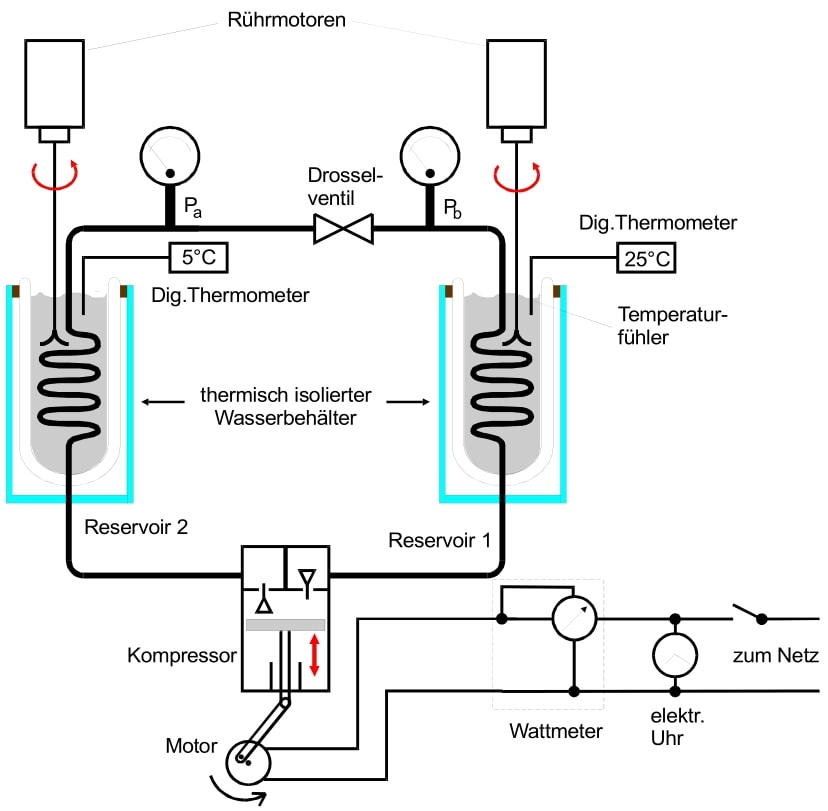
\includegraphics[width=0.75\linewidth]{./images/Aufbau.jpg}
        \caption{Aufbau der Röntgenröhre \cite{V603}}
        \label{fig:1}
    \end{figure}

    \flushleft{Zu\;}\justifying Beginn wird der LiF-Kristall in die Halterung gesteckt und eine $\SI{2}{\milli\meter}$-Blende verwendet. Das RS232-Kabel wird angeschlossen, wie auf
    Abbildung \ref{fig:1} gezeigt. Um das Emissionsspektrum der Kupfer-Röntgenröhre 
    zu bestimmen, wird das Röntgenspektrum im $\SI{10}{\second}$-Intervall abgelesen, wobei der Einfallwinkel nach jeder Messung um $0.1°$ variiert wird.
    Hier wurde die Messung bei einem Winkel $\alpha = 8°$ begonnen und bei $\alpha = 25°$ abgeschlossen. 

    \flushleft{Anschließend\;}\justifying wird die Transmission des Aluminiumabsorbers gemessen, indem der Aluminiumabsorber vor die $\SI{2}{\milli\meter}$-Blende gelegt, das RS232-Kabel
    abgeogen und der Einfallwinkel um 0.1° über $\SI{200}{\second}$ variiert wird. Hier ist der Startwinkel $\alpha = 7°$ und die Messung wurde bei $\alpha = 10°$ beendet. 
    Mithilfe der Messwerte wird ein $\lambda$-$T$ Diagramm erstellt. Für die Transmission wird die Intensität der Strahlung benötigt, welche sich mit der vorliegenden
    Totzeit des Geiger-Müller Zählrohrs von $\tau = \SI{90}{\micro\second}$ bestimmen lässt. 

    \begin{figure}
        \centering
        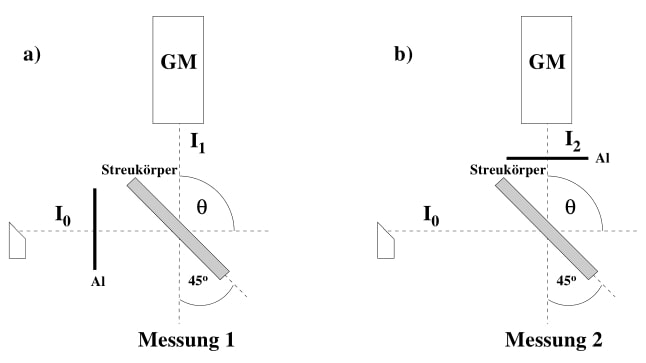
\includegraphics[width=0.75\linewidth]{./images/Aufbau2.jpg}
        \caption{Versuchsaufbau \cite{V603}}
        \label{fig:1b}
    \end{figure}

    \flushleft{Um\;}\justifying die Compton-Wellenlänge zu bestimmen, soll die Intensität der Kupfer-Röhre $I_0$ bestimmt werden. Dazu wird die $\SI{2}{\milli\meter}$-Blende
    durch eine $\SI{5}{\milli\meter}$-Blende und der LiF-Kristall durch den Plexiglas-Streuer ersetzt. Der Kristall wird auf 45° und das Geiger-Müller Zählrohr auf 90° gestellt, 
    wie in Abbildung \ref{fig:1b} dargestellt. Mit diesen Einstellung wird die Intensität $I_0$ abgelesen.

    \flushleft{Für\;}\justifying die Compton-Wellenlänge werden die verbleibenden Intensitäten $I_1$ und $I_2$ der Strahlung bestimmt. Dafür wird der Aluminiumabsorber 
    einmal zwischen Röntgenröhre und Streukörper $I_1$ und einmal zwischen Streukörper und Geiger-Müller Zählrohr $I_2$ gesteckt, wie in Abbildung \ref{fig:1b} dargestellt. 
    Beide Messungen werden unabhängig über einen Zeitraum $\SI{300}{\second}$ und einem Winkelintervall von $7° \leq \alpha \leq 10°$ durchgeführt. 


\newpage
\section{Auswertung}

    \subsection{Emissionsspektrum von Kupfer}

    \flushleft{Alle\;}\justifying folgenden Graphen werden mit der python Bibliothek matplotlib \cite{matplotlib} erstellt.
    Mithilfe der Messwerte aus Tabelle \ref{tab:1} wird das Emissionsspektrum von Kupfer graphisch aufgetragen:

    \begin{figure}[H]
        \centering
        \includegraphics[width=\linewidth]{plotCu.pdf}
        \caption{Emissionsspektrum der Kupferröhre}
        \label{fig:2}
    \end{figure}

    \flushleft{Anhand\;}\justifying des Graphen lassen sich die Werte der Winkel für die $K_{\alpha}$- und $K_{\beta}$-Linie ablesen. Diese lauten:
    \begin{align}
        Winkel_{K_{\alpha}} &= \text{\input{xmax.tex}}  \label{eq:5}\\
        Winkel_{K_{\beta}}  &= \text{\input{xlmax.tex}} \label{eq:6}
    \end{align}
    Wobei hier der Fehler \SI{0.1}{\degree} beträgt.

    \flushleft{Mit\;}\justifying den Winkeln \eqref{eq:5} und \eqref{eq:6} und der Gleichung \eqref{eq:2} lassen sich die Wellenlängen $\lambda_{\alpha}$ und $\lambda_{\beta}$ bestimmen,
    welche für $\lambda$ in die Formel der Energie \eqref{eq:3} eingesetzt werden. Die Wellenlängen der $K_{\alpha}\,$- und der $K_{\beta}\,$-Linie lauten:
    \begin{align}
    \lambda_{\alpha} &= \text{\input{L_a.tex}}  \label{eq:8}\\
    \lambda_{\beta} &= \text{\input{L_b.tex}}   \label{eq:9}
    \intertext{
        \flushleft{Werden\;}\justifying diese Werte in Gleichung \eqref{eq:3} eingesetzt, ergibt sich für die Energie der jeweiligen Linie:
    }
    E_{\alpha} &= \text{\input{E_a.tex}}    \label{eq:10}\\
    E_{\beta} &= \text{\input{E_b.tex}.}     \label{eq:11}
    \end{align}
    
    \subsection{Transmission von Aluminium}

    \flushleft{Um\;}\justifying die Transmission $T$ von Aluminium zu bestimmen, wird zuerst die Intensität $I$ bestimmt. Diese lässt sich mit der Formel \eqref{eq:4}
    bestimmen. Die Totzeit des Geiger-Müller Zählrohrs $\tau$ ist hier $\SI{90}{\micro\second}$. Außerdem ist hier die Poissonverteilung
    Der Impulsraten wichtig, welche einen Fehler $\Delta N = \sqrt{N}$ mit sich zieht.

    \flushleft{Werden\;}\justifying die Werte für Impulse pro Sekunde aus Tabelle \ref{tab:2} für $N$ in Gleichung \eqref{eq:4} eingesetzt, ergeben sich die folgenden Intensitäten:
    \begin{align}
        I_1 &= \frac{N_0}{1- \tau \cdot N_0}   \label{eq:12}\\
        I_2 &= \frac{N_{Al}}{1- \tau \cdot N_{Al}} \label{eq:13}
    \end{align}

    \flushleft{Mit\;}\justifying $I_1$ \eqref{eq:12}, $I_2$ \eqref{eq:13} und der Formel \eqref{eq:T} lässt sich nun die Transmission bestimmen. Für das folgende $\lambda$-T Diagramm
    ist die Wellenlänge $\lambda$ wichtig, welche sich wie zuvor mit Gleichung \eqref{eq:2} bestimmen lässt. Mit der Geradengleichung 
    \begin{align}
    T = m \cdot x + b, \label{eq:14}
    \end{align}
    dem python Befehl np.polyfit 
    \cite{numpy} und den dazugehörigen Parametern
    \begin{align}
        m &= \text{\input{m_Al.tex}} \label{eq:15}\\
        b &= \text{\input{b_Al.tex}} \label{eq:16}
    \end{align}
    lässt sich die folgende lineare Regression erstellen:

    \begin{figure}[H]
        \centering
        \includegraphics[width=0.75\linewidth]{plotAl.pdf}
        \caption{Lineare Regression der Transmission des Aluminiumabsorbers}
        \label{fig:3}
    \end{figure}

    \subsection{Compton-Wellenlänge}

    \flushleft{Die\;}\justifying Compton-Wellenlänge eines Elektrons $\lambda_C$ wird mit der umgestellten Formel \eqref{eq:2} nach $\lambda$ bestimmt:
    \begin{align}
        \lambda = 2 \cdot d \cdot \sin(\alpha) \qquad \qquad \text{für $n\,=\,1$} \label{eq:17}
    \end{align} 
    Für die Transmissionen
    \begin{align}
        T_1 &= \sfrac{I_1}{I_0} \\
        T_2 &= \sfrac{I_2}{I_0} 
    \end{align}
    werden die Intensitäten $I_0$, $I_1$, und $I_2$ benötigt. Diese werden aus der Versuchsanleitung \cite{V603} übernommen:
    \begin{subequations}\label{eq:18}
    \begin{align}
        I_0 &= \text{\input{I_0.tex}} \label{eq:18a}\\
        I_1 &= \text{\input{I_1.tex}} \label{eq:18b}\\
        I_2 &= \text{\input{I_2.tex}} \label{eq:18c}
    \end{align}
    \end{subequations}

    \flushleft{Die\;}\justifying daraus resultierenden Transmissionen ergeben:
    \begin{align}
        T_1 &= \text{\input{T_1.tex}} \label{eq:19}\\
        T_2 &= \text{\input{T_2.tex}} \label{eq:20}
    \end{align}

    \flushleft{Mit\;}\justifying $T_1$, $T_2$ und der Formel
    \begin{align}
        \lambda = \frac{T - b}{m},
    \end{align}
    welche sich aus der Geradengleichung \eqref{eq:14} ergibt, lassen sich die Wellenlängen $\lambda_1$ und $\lambda_2$ berechnen:
    \begin{align}
        \lambda_1 &= \text{\input{L_1.tex}}\\
        \lambda_2 &= \text{\input{L_2.tex}}
    \end{align} 
    Dessen Differenz $\Delta \lambda$ ergibt nach Formel \eqref{eq:1} die Compton-Wellenlänge $\lambda_C$.
    Demnach ergibt sich für $\lambda_C$:
    \begin{align}
        \lambda_C = \text{\input{L_C.tex}} \label{eq:21}
    \end{align}


\newpage
\section{Diskussion}

    \flushleft{In\;}\justifying der folgenden Tabelle \ref{tab:3} sind die erarbeiteten Werte, die Literaturwerte und dessen relative Fehler zu finden: 

    \begin{table}[H]
    \centering
        \begin{tabular}{l c c r}
            \toprule
            \multicolumn{1}{c}{} & \multicolumn{1}{c}{Messwerte} & \multicolumn{1}{c}{Literaturwerte} & \multicolumn{1}{c}{Relativer Fehler}\\
            \cmidrule(lr{0,5em}){1-4}
            $E_{\alpha}$           & \input{E_a.tex}            & \input{E_a_lit.tex} \cite{NIST}            & \input{E_Fa.tex} \\
            $E_{\beta}$            & \input{E_b.tex}            & \input{E_b_lit.tex} \cite{NIST}            & \input{E_Fb.tex} \\
            $\lambda_C$            & \input{L_C.tex}            & \input{L_const.tex} \cite{scipy}           & \input{L_C_F.tex} \\
            \bottomrule
        \end{tabular}
    \caption{Messwertvergleich mit den jeweiligen Literaturwerten}
    \label{tab:3}
    \end{table}

    \flushleft{Aus\;}\justifying den relativen Fehlern der Tabelle \ref{tab:3} für $K_{\alpha}$ und $K_{\beta}$ lässt sich ein deutliches Verhältniss zwischen der
    erwarteten Kurve und der gemessenen Kurve feststellen. Der Graph \ref{fig:2} gibt die Peaks der $K_{\alpha}$- und $K_{\beta}$-Linie deutlich und mit geringem 
    Fehler wieder. 

    \flushleft{Der\;}\justifying Graph \ref{fig:3} veranschaulicht die Linearität der Transmission des Aluminiumabsorbers im Verhältniss zur Wellenlänge. Dieses Verhältniss
    wird von dem relativ geringen Fehlern der Parameter \eqref{eq:15} und \eqref{eq:16} gestärkt. 

    \flushleft{Bei\;}\justifying der Compton-Wellenlänge $\lambda_C$ hingegen entsteht ein signifikanter Fehler von $\SI{55}{\percent}$. Es wird mit der Bragg´schen Bedingung \eqref{eq:2} 
    angenommen, dass es sich bei der atomaren Struktur, des Streukristalls um ein perfekt symmetrisches Gitternetz handelt. Dies ist in der Regel jedoch nicht der Fall, da Kristalle auf atomarer
    Ebene nicht perfekt geschliffen werden können und Abnutzung das Gitternetz weiter beschädigt. Diese Verunreinigungen können dazu führen, dass die Röntgenstrahlung unterschiedlich gestreut wird, 
    wodurch unterschiedliche Wellenlängen erzeugt werden. Außerdem können Unreinheiten ebenfalls im Vakuum und auf der Anode entstehen. Da es nicht möglich ist ein perfektes Vakuum künstlich herzustellen, 
    können Restatome die Röntgenstrahlung beeinflusst haben. Kollision mit Teilchen spielt auch in der Streuvorrichtung selbst eine Rolle, da, wie in Abbildung \ref{fig:1} zu erkennen ist, sich der 
    Streuer \circled{3} nicht im Vakuum befindet. Dies kann zu einer Ionisierung der Luft führen, welche wiederum die gemessene Intensität beeinflusst, indem neue Wellenlängen gemessen werden.  

\newpage
\printbibliography

\newpage
\section{Appendix}

\input{table_Cu.tex}

\input{table_Al.tex}

\end{document}